\documentclass[12pt,fleqn]{exam}
\usepackage{pifont}
\usepackage{dingbat}
\usepackage{amsmath,amssymb}
\usepackage{epsfig}
\usepackage[colorlinks=true,linkcolor=black,anchorcolor=black,citecolor=black,filecolor=black,menucolor=black,runcolor=black,urlcolor=black]{hyperref}
\usepackage[letterpaper, margin=0.75in]{geometry}
\addpoints
\boxedpoints
\pointsinmargin
\pointname{pts}

\usepackage[final]{microtype}
\usepackage[american]{babel}
\usepackage[T1]{fontenc}
\usepackage{fourier}
\usepackage{isomath}
\usepackage{upgreek,amsmath}
\usepackage{amssymb}

\newcommand{\dotprod}{\, {\scriptzcriptztyle
    \stackrel{\bullet}{{}}}\,}

\newcommand{\reals}{\mathbf{R}}
\newcommand{\lub}{\mathrm{lub}} 
\newcommand{\glb}{\mathrm{glb}} 
\newcommand{\complex}{\mathbf{C}}
\newcommand{\dom}{\mbox{dom}}
\newcommand{\range}{\mbox{range}}
\newcommand{\cover}{{\mathcal C}}
\newcommand{\integers}{\mathbf{Z}}
\newcommand{\vi}{\, \mathbf{i}}
\newcommand{\vj}{\, \mathbf{j}}
\newcommand{\vk}{\, \mathbf{k}}
\newcommand{\bi}{\, \mathbf{i}}
\newcommand{\bj}{\, \mathbf{j}}
\newcommand{\bk}{\, \mathbf{k}}
\newcommand{\dist}{\, \mathrm{dist}}
\DeclareMathOperator{\Arg}{\mathrm{Arg}}
\DeclareMathOperator{\Ln}{\mathrm{Ln}}
\newcommand{\imag}{\, \mathrm{i}}

\usepackage{xcolor}
\shadedsolutions
\definecolor{SolutionColor}{rgb}{0.95,0.95,0.95}

\usepackage{graphicx}
\newcommand\AM{{\sc am}}
\newcommand\PM{{\sc pm}}
     
%\usepackage{twemojis}
\newcommand{\quiz}{5}
\newcommand{\term}{Spring}
\newcommand{\due}{9:55 \AM}
\newcommand{\class}{MATH 102}
\begin{document}
\large
\vspace{0.1in}
\noindent\makebox[3.0truein][l]{\textbf{\class, \term \/ \the\year}}
\textbf{Name:} \hrulefill \\
\noindent \makebox[3.0truein][l]{\textbf{In class work \quiz}}
\textbf{Row and Seat}:\hrulefill\\
\vspace{0.1in}


\noindent  In class work  \quiz\/  has questions 1 through  \numquestions \/ with a total of  \numpoints\/  points.   
 This assignment is due at the end of the class period (\due).

\vspace{0.1in}


\begin{questions} 

    \question [5] Find the \emph{distance} between the points $(7,2)$ and $(-1,-2)$.
    \begin{solution}[2.0in]
    We have
    \begin{align*}
        \dist((7,2),(-1,-2)) &= \sqrt{(7+1)^2 + (2 + 2)^2}, &(\mbox{distance formula})\\
                               &= \sqrt{64+ 16}, &(\mbox{arithmetic})\\
                               &= \sqrt{80}, &(\mbox{arithmetic}) \\
                               &= 4 \sqrt{5}.
    \end{align*}
    
    
    \end{solution}

  \question [5] Find the \emph{midpoint} of the points $(2,4)$ and $(5,7)$.
  \begin{solution}[2.0in]
  \end{solution}

  \question[5] A line $L$ contains the points $(x=5,y=7)$ and
$(x=7,y=-1)$.  

\begin{parts}

    \part [5] Find an \emph{equation} of the line $L$.
    \begin{solution}[1.5in] 
    \end{solution}

    \part  [5] Find the \emph{x-intercept} of the line $L$.
    \begin{solution}%[1.5in] 
    \end{solution}

\end{parts}

\newpage


\question [5] Find an equation of the line that is parallel to the
line $3 y + 6 x = 1$ and that contains the point $(x=1,y=1)$.
\begin{solution}[1.5in] 
\end{solution}

\question [5] Find the \emph{center} and \emph{radius} of the circle
\(
   x^2 + 2 x + y^2 - 6 y = -6.
\)

\begin{solution}[2.4in]
\end{solution}

\question [5] The number of doghouses $L$ a work crew can build
 in a day varies jointly with the number of people $N$ in the crew and with
the time $T$  they work in a day. Given that $L = 12$ when $N = 5$ and $T = 6$, find $L$ when
$N = 20$ and $T = 10$.
\begin{solution}%[3.5in]


\end{solution}
\newpage

\question Shown below is a graph of the equation $y = U(x)$. 
Some points on the graph are labeled. The domain of $U$ is
the closed interval $[-2,2]$

\begin{figure}[h]
    \begin{center}
    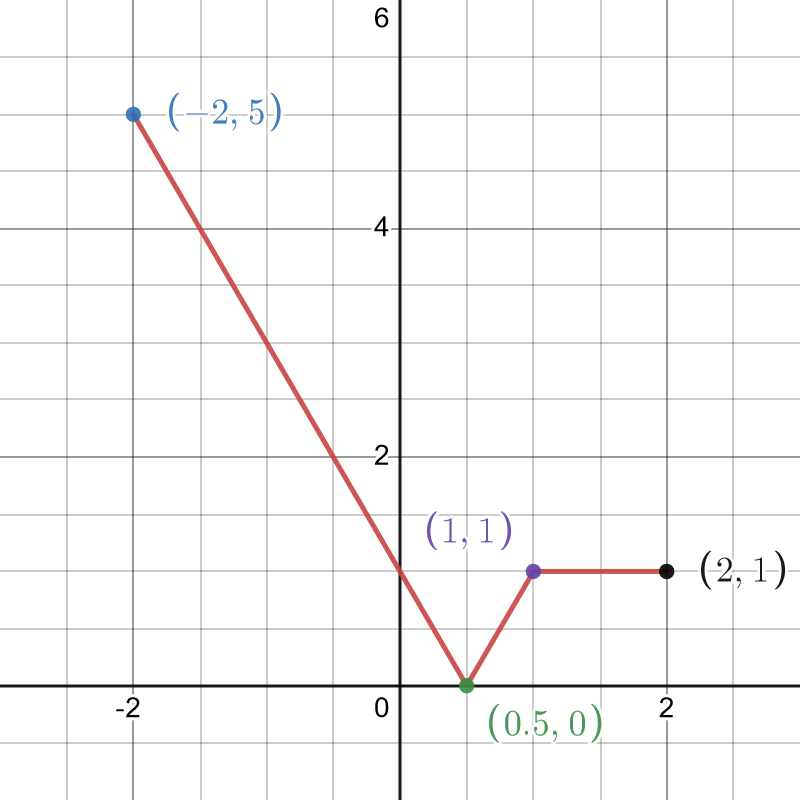
\includegraphics[scale=0.2]{desmos-graph(14).png}
\end{center}
\caption{Graph of the equation$y = U(x)$.}
\end{figure}

\begin{parts}

\part [5] Find the numerical value of $U(-2)$.
\begin{solution}[0.5in]

\end{solution}

\part [5] Find the \emph{range} of $U$.
\begin{solution}[2.3in]

\end{solution}

\part [5] Find the interval(s) on which $U$ is \emph{decreasing.}
\begin{solution}[2.3in]

\end{solution}

\part [5] Find the interval(s) on which $U$ is \emph{increasing.}
\begin{solution}[2.3in]

\end{solution}

\part [5] Find the interval(s) on which $U$ is \emph{constant.}
\begin{solution}[2.3in]

\end{solution}

\part [5] Sketch a graph of the equation $y-1 = U(x-1)$.
\begin{solution}%[2.3in]

\end{solution}

\end{parts}

\newpage
\question Define a function $Q$ by $Q(x) = \begin{cases}  x &  x < 1 \\   5 &  1 \leq x \end{cases}$.

\begin{parts}
\part [5]  Find the numerical value of $Q(-2)$.
\begin{solution}[2.3in]

\end{solution}

\part [5]  Find the numerical value of $Q(2)$.
\begin{solution}[2.3in]

\end{solution}

\part [5] Sketch a graph of $Q$.
\begin{solution}[2.3in]

\end{solution}

\part Find the \emph{average rate of change} of $Q$ on the interval $[-2,2]$.




\end{parts}

\end{questions}
\end{document}
